\documentclass[10pt]{exam}
\usepackage[phy]{template-for-exam}
\usepackage{tikz}
\usepackage[top=0.2in, bottom=0.5in, left=1in, right=1in]{geometry}


\begin{document}
\pagestyle{empty}

\def\mytitle{Unit 06 Test: Momentum}

\newcommand{\topmatter} {

  \hrule \vspace{1em}

  \noindent {\bf Please do not open this test until told to do so!}

  \begin{itemize}
    \item Put your name on both this page and the next page.
    \item Bubble in the number that is on your class notebook where it says “Student ID”
    \item When instructed, tear off this first page.
    \item Write your answers to the free-response questions directly on the packet.
    \item Bubble in your answers to the multiple-choice questions here.
    \item You may write anywhere on the packet.
    
  \end{itemize}


  \vspace{4em}

  \begin{center}
    \begin{tabular}{|*{11}{c}|}
      \hline 
      &&&&&&&&&&\\
      &
      $W=Fd$ &&
      $P=\frac{W}{t}$ &&
      $F_G=mg$ &&
      $KE=\frac{1}{2}mv^2$ &&
      $PE=mgh$ &\\
      &&&&&&&&&&\\
      \multicolumn{11}{|c|}{$KE_i + PE_i + W = KE_f + PE_f$}\\
      &&&&&&&&&&\\
      \hline
    \end{tabular}
  \end{center}

}
\newcommand{\bottommatter}{
}

\newcommand{\drawscantron}[2]{
  \begin{flushright}
    \begin{tikzpicture}[scale=0.8]
      \node[anchor=south west] at (0,0) {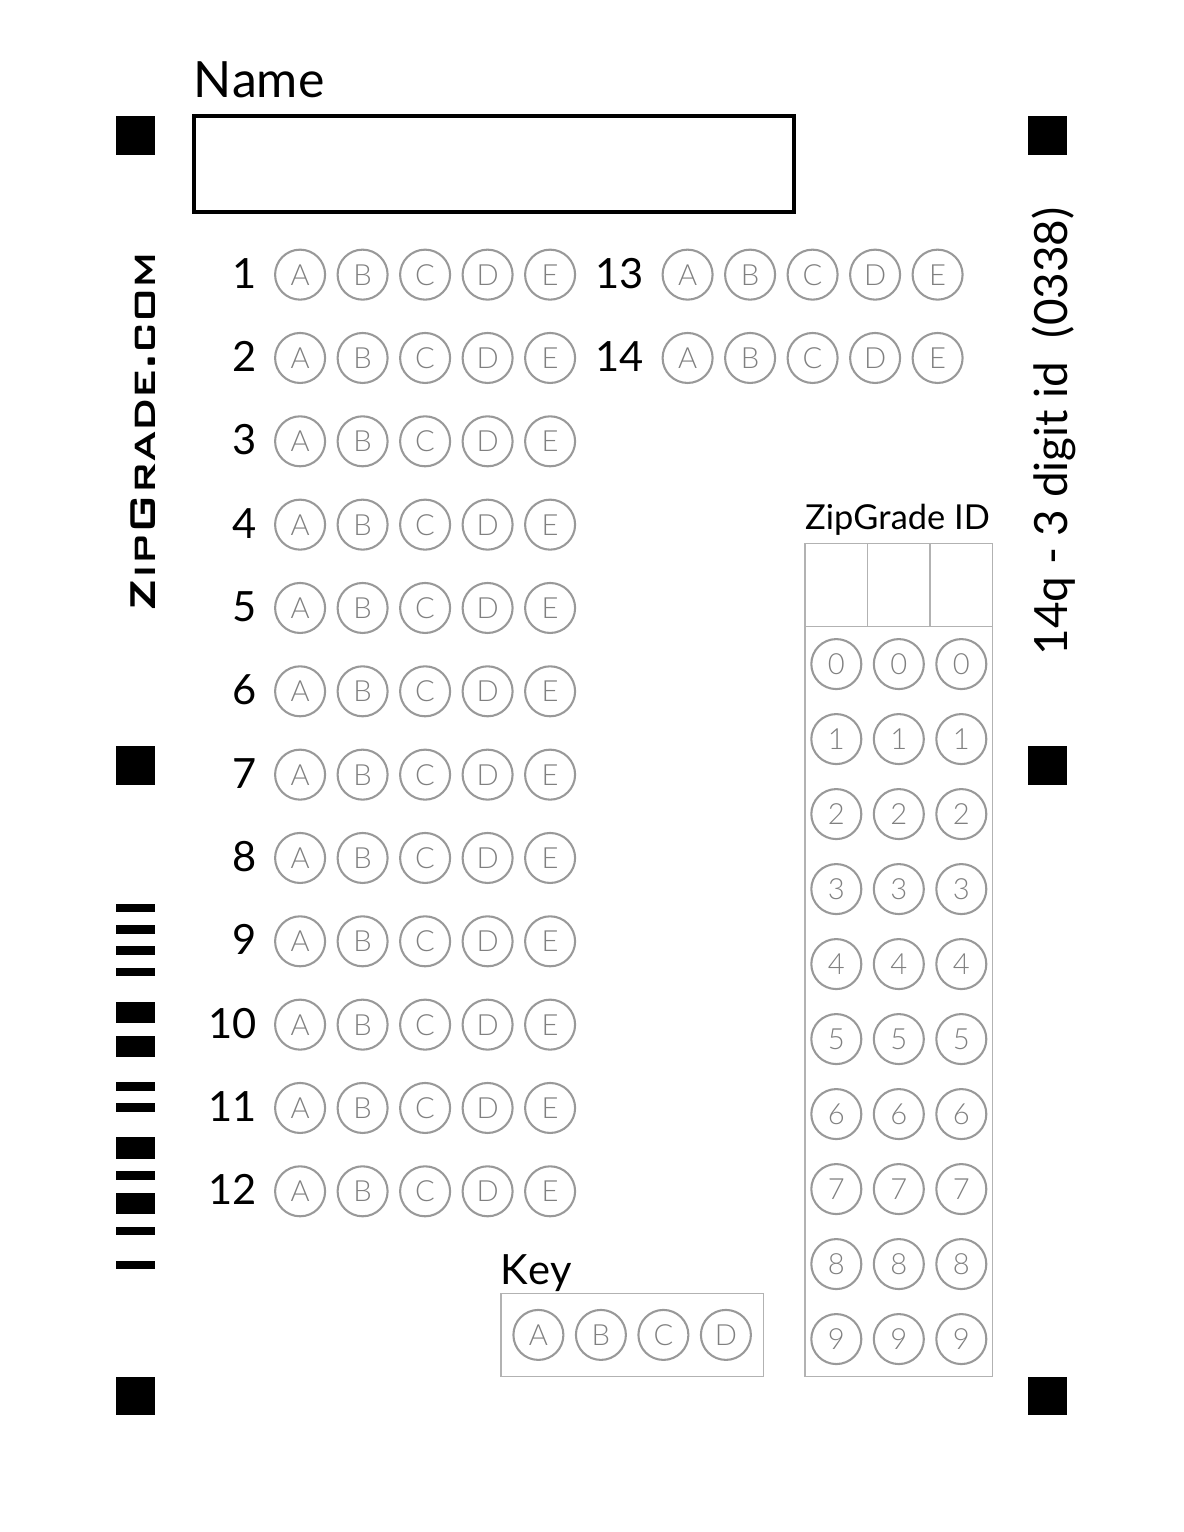
\includegraphics[width=.56\textwidth]{14Q.png}};
      \fill (#1,#2) circle (0.25);
    \end{tikzpicture}
  
    \bottommatter
  \end{flushright}
}



  \drawscantron{5.4}{2.1}
  \topmatter

\pagebreak

  \drawscantron{6}{2.1}
  \topmatter



\end{document}